\chapter{Feature Analysis}

\section{Extracting utilizations from github repositories containing python}
Our goal was to collect regexes from a variety of projects to represent the breadth of how developers use the language features.
Using the GitHub API, we scraped \dbfetch{nProjScanned} projects containing Python code.
We did so  by dividing a range of about 8 million repo IDs
into 32 sections of equal size and scanning  for Python projects from the beginning of those
segments until we ran out of memory. At that point, we felt we had enough data
to do an analysis without further perfecting our mining techniques. We built
the AST of each Python file in each project to find utilizations of the {\tt re} module
functions. In most projects, almost all regex utilizations are present in the
most recent version of a project, but to be more thorough, we also scanned up
to 19 earlier versions. The number 20 was chosen to try and maximize returns on
computing resources invested after observing the scanning process in many hours
of trial scans.
All regex utilizations were obtained, sans duplicates. Within a project, a duplicate utilization was marked when two versions of the same file have the same function, pattern and flags.  In the end, we observed and recorded \dbfetch{nUsages} non-duplicate regex utilizations in \dbfetch{nProjScanned} projects.

In collecting the set of distinct patterns for analysis,  we ignore the \dbfetch{percentBadFlags}\%  of utilizations using flags, which can alter regex behavior.  An additional \dbfetch{percentInvalidPattern}\% of utilizations contained patterns that could not be compiled because the pattern was non-static (e.g., used some runtime variable).
The remaining \dbfetch{percentCleanUsages}\% (\dbfetch{nCleanUsages}) of the utilizations were collapsed into \dbfetch{nDistinctPatterns} distinct pattern strings.  Each of the pattern strings was pre-processed by removing Python quotes (\verb!`\\W!' becomes \verb!\\W!), unescaping escaped characters (\verb!\\W! becomes \verb!\W!) and parsing the resulting  string using an ANTLR-based, open source PCRE parser\footurl{https://github.com/bkiers/pcre-parser}.
This parser was unable to support \dbfetch{percentUnicode}\% (\dbfetch{N_UNICODE}) of the patterns due to unsupported unicode characters.  Another \dbfetch{percentAlien}\% (\dbfetch{N_ALIEN}) of the patterns used regex features that we  chose to exclude because they appeared very rarely (e.g., reference conditions).  An additional 0.1\% (16) of the patterns were excluded because they were empty or otherwise malformed so as to cause a parsing error.

The \dbfetch{nCorpus} distinct pattern strings that remain were each assigned a weight value equal to the number of distinct projects the pattern appeared in.  We  refer to this set of weighted, distinct pattern strings as the \emph{corpus}.

\subsection{Experiment design}
Third, we investigate what features are supported by four large projects that aim to support regex usage (brics~\cite{brics}, hampi~\cite{hampi}, Rex~\cite{rex}, and RE2~\cite{re2}), and which features are not supported, but are frequently used by developers.

\subsection{Implementation details}


\section{Utilizations of the re module}
We explore regex utilizations and flags used in the scraped Python projects.
Out of the \dbfetch{nProjScanned}\ projects scanned, \dbfetch{percentProjectsUsingRegex}\% (\dbfetch{nProjectsUsingRegex}) contained at least one regex utilization.  To illustrate how saturated projects are with regexes, we measure utilizations per project, files scanned per project, files contained utilizations, and  utilizations  per file, as shown in Table~\ref{table:saturation}.

Of projects containing at least one utilization, the average utilizations per project was 32 and the maximum  was 1,427.  The project with the most utilizations is a C\# project\footurl{https://github.com/Ouroboros/Arianrhod} that maintains a collection of source code for 20 Python libraries, including larger libraries like {\tt pip}, {\tt celery} and {\tt ipython}.  These larger Python libraries contain many utilizations.
From Table~\ref{table:saturation}, we also see that each project had an average of 11 files containing any utilization, and each of these files had an average of 2 utilizations.

\begin{figure}[tb]
\centering
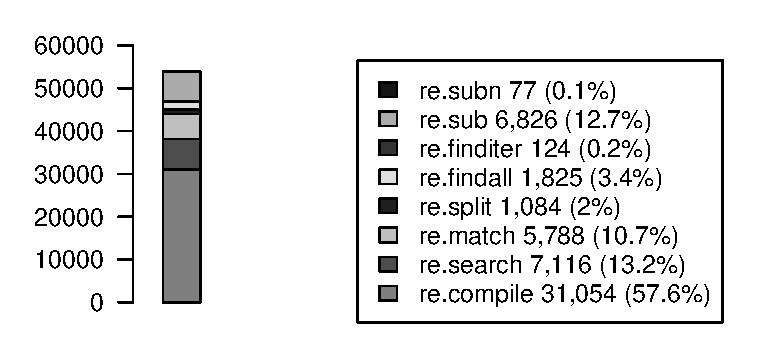
\includegraphics[width=\columnwidth]{nontex/illustrations/partFunctions.eps}
\vspace{-12pt}
\caption{How often are  {\tt re} functions used? (RQ2)}
\vspace{-6pt}
\label{fig:partFunctions}
\end{figure}

\begin{figure}[tb]
\centering
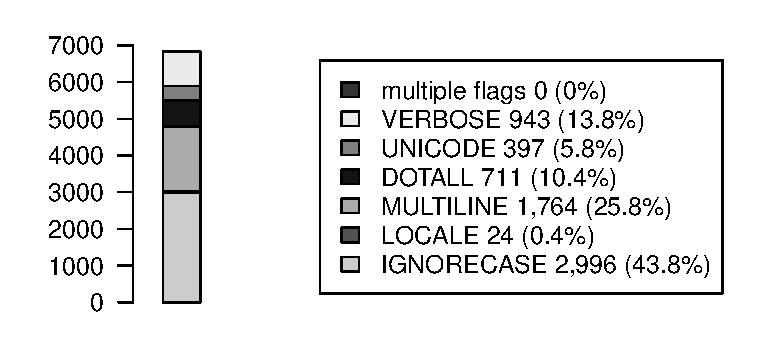
\includegraphics[width=0.9\columnwidth]{nontex/illustrations/partFlags.eps}
\vspace{-6pt}
\caption{Which behavioral flags are used? (RQ2)}
\vspace{-6pt}
\label{fig:partFlags}
\end{figure}


\section{Building the corpus of patterns}
\subsection{Experiment design}
\subsection{Implementation details}

\section{Features of patterns in the corpus}
For each escaped pattern, the PCRE-parser produces a tree of feature tokens, which is converted to a vector by counting the number of each token  in the tree.  For a simple example, consider the patterns in Figure~\ref{fig:featureParsing}.  The pattern \verb!`^m+(f(z)*)+'! contains four different types of tokens. It has the kleene star (KLE), which is specified using the asterisk \verb!`*'! character, additional repetition (ADD), which is specified using the plus \verb!`+'! character, capture groups (CG), which are specified using pairs of parenthesis \verb!`(...)'! characters, and the start anchor (STR), which is specified using the caret \verb!`^'! character at the beginning of a pattern. A list of all features and abbreviations is provided in Table~\ref{table:featureStats}.

\begin{figure}[tb]
\centering

\includegraphics[height=0.6in]{nontex/illustrations/featureParsing.eps}
\caption{Two patterns parsed into feature vectors}
\label{fig:featureParsing}
\vspace{-12pt}
\end{figure}

Once all patterns were transformed into vectors, we examined each feature independently for all patterns, tracking the number of patterns and  projects that the each feature appears in at least once.

\begin{table*}
\begin{center}
\caption{How Frequently do Features Appear in Projects, and Which Features are Supported By Four Major Regex Projects? (RQ2)}
\label{table:featureStats}
\begin{tabular}
{llllcccccccccc}
rank & code & description & example & brics & hampi & Rex & RE2 & nPatterns & \% patterns & nProjects & \% projects \\ 
\toprule[0.16em]
1 & ADD & one-or-more repetition & \begin{minipage}{0.5in}\begin{verbatim}z+\end{verbatim}\end{minipage} & \yes & \yes & \yes & \yes & 6,003 & 44.1 & 1,204 & 73.2 \\ 
\midrule
2 & CG & a capture group & \begin{minipage}{0.5in}\begin{verbatim}(caught)\end{verbatim}\end{minipage} & \yes & \yes & \yes & \yes & 7,130 & 52.4 & 1,194 & 72.6 \\ 
\midrule
3 & KLE & zero-or-more repetition & \begin{minipage}{0.5in}\begin{verbatim}.*\end{verbatim}\end{minipage} & \yes & \yes & \yes & \yes & 6,017 & 44.3 & 1,099 & 66.8 \\ 
\midrule
4 & CCC & custom character class & \begin{minipage}{0.5in}\begin{verbatim}[aeiou]\end{verbatim}\end{minipage} & \yes & \yes & \yes & \yes & 4,468 & 32.9 & 1,026 & 62.4 \\ 
\midrule
5 & ANY & any non-newline char & \begin{minipage}{0.5in}\begin{verbatim}.\end{verbatim}\end{minipage} & \yes & \yes & \yes & \yes & 4,657 & 34.3 & 1,005 & 61.1 \\ 
\midrule
6 & RNG & chars within a range & \begin{minipage}{0.5in}\begin{verbatim}[a-z]\end{verbatim}\end{minipage} & \yes & \yes & \yes & \yes & 2,631 & 19.3 & 848 & 51.6 \\ 
\midrule
7 & STR & start-of-line & \begin{minipage}{0.5in}\begin{verbatim}^\end{verbatim}\end{minipage} & \no & \yes & \yes & \yes & 3,563 & 26.2 & 846 & 51.4 \\ 
\midrule
8 & END & end-of-line & \begin{minipage}{0.5in}\begin{verbatim}$\end{verbatim}\end{minipage} & \no & \yes & \yes & \yes & 3,169 & 23.3 & 827 & 50.3 \\ 
\midrule[0.12em]
9 & NCCC & negated CCC & \begin{minipage}{0.5in}\begin{verbatim}[^qwxf]\end{verbatim}\end{minipage} & \yes & \yes & \yes & \yes & 1,935 & 14.2 & 776 & 47.2 \\ 
\midrule
10 & WSP & \textbackslash t \textbackslash n \textbackslash r \textbackslash v \textbackslash f or space & \begin{minipage}{0.5in}\begin{verbatim}\s\end{verbatim}\end{minipage} & \no & \yes & \yes & \yes & 2,846 & 20.9 & 762 & 46.3 \\ 
\midrule
11 & OR & logical or & \begin{minipage}{0.5in}\begin{verbatim}a|b\end{verbatim}\end{minipage} & \yes & \yes & \yes & \yes & 2,102 & 15.5 & 708 & 43 \\ 
\midrule
12 & DEC & any of: 0123456789 & \begin{minipage}{0.5in}\begin{verbatim}\d\end{verbatim}\end{minipage} & \no & \yes & \yes & \yes & 2,297 & 16.9 & 692 & 42.1 \\ 
\midrule
13 & WRD & [a-zA-Z0-9\_] & \begin{minipage}{0.5in}\begin{verbatim}\w\end{verbatim}\end{minipage} & \no & \yes & \yes & \yes & 1,430 & 10.5 & 650 & 39.5 \\ 
\midrule
14 & QST & zero-or-one repetition & \begin{minipage}{0.5in}\begin{verbatim}z?\end{verbatim}\end{minipage} & \yes & \yes & \yes & \yes & 1,871 & 13.8 & 645 & 39.2 \\ 
\midrule
15 & LZY & as few reps as possible & \begin{minipage}{0.5in}\begin{verbatim}z+?\end{verbatim}\end{minipage} & \no & \yes & \no & \yes & 1,300 & 9.6 & 605 & 36.8 \\ 
\midrule
16 & NCG & group without capturing & \begin{minipage}{0.5in}\begin{verbatim}a(?:b)c\end{verbatim}\end{minipage} & \no & \yes & \no & \yes & 791 & 5.8 & 404 & 24.6 \\ 
\midrule
17 & PNG & named capture group & \begin{minipage}{0.5in}\begin{verbatim}(?P<name>x)\end{verbatim}\end{minipage} & \no & \yes & \no & \yes & 915 & 6.7 & 354 & 21.5 \\ 
\midrule
18 & SNG & exactly n repetition & \begin{minipage}{0.5in}\begin{verbatim}z{8}\end{verbatim}\end{minipage} & \yes & \yes & \yes & \yes & 581 & 4.3 & 340 & 20.7 \\ 
\midrule
19 & NWSP & any non-whitespace & \begin{minipage}{0.5in}\begin{verbatim}\S\end{verbatim}\end{minipage} & \no & \yes & \yes & \yes & 484 & 3.6 & 270 & 16.4 \\ 
\midrule
20 & DBB & $n\le x \le m$ repetition & \begin{minipage}{0.5in}\begin{verbatim}z{3,8}\end{verbatim}\end{minipage} & \yes & \yes & \yes & \yes & 367 & 2.7 & 238 & 14.5 \\ 
\midrule
21 & NLKA & sequence doesn't follow  & \begin{minipage}{0.5in}\begin{verbatim}a(?!yz)\end{verbatim}\end{minipage} & \no & \no & \no & \no & 131 & 1 & 183 & 11.1 \\ 
\midrule
22 & WNW & word/non-word boundary & \begin{minipage}{0.5in}\begin{verbatim}\b\end{verbatim}\end{minipage} & \no & \no & \no & \yes & 248 & 1.8 & 166 & 10.1 \\ 
\midrule
23 & NWRD & non-word chars & \begin{minipage}{0.5in}\begin{verbatim}\W\end{verbatim}\end{minipage} & \no & \yes & \yes & \yes & 94 & 0.7 & 165 & 10 \\ 
\midrule
24 & LWB & at least n repetition & \begin{minipage}{0.5in}\begin{verbatim}z{15,}\end{verbatim}\end{minipage} & \yes & \yes & \yes & \yes & 91 & 0.7 & 158 & 9.6 \\ 
\midrule
25 & LKA & matching sequence follows & \begin{minipage}{0.5in}\begin{verbatim}a(?=bc)\end{verbatim}\end{minipage} & \no & \no & \no & \no & 112 & 0.8 & 158 & 9.6 \\ 
\midrule
26 & OPT & options wrapper & \begin{minipage}{0.5in}\begin{verbatim}(?i)CasE\end{verbatim}\end{minipage} & \no & \yes & \no & \yes & 231 & 1.7 & 154 & 9.4 \\ 
\midrule
27 & NLKB & sequence doesn't precede & \begin{minipage}{0.5in}\begin{verbatim}(?<!x)yz\end{verbatim}\end{minipage} & \no & \no & \no & \no & 94 & 0.7 & 137 & 8.3 \\ 
\midrule[0.12em]
28 & LKB & matching sequence precedes & \begin{minipage}{0.5in}\begin{verbatim}(?<=a)bc\end{verbatim}\end{minipage} & \no & \no & \no & \no & 80 & 0.6 & 120 & 7.3 \\ 
\midrule
29 & ENDZ & absolute end of string & \begin{minipage}{0.5in}\begin{verbatim}\Z\end{verbatim}\end{minipage} & \no & \no & \no & \yes & 89 & 0.7 & 90 & 5.5 \\ 
\midrule
30 & BKR & match the $i^{th}$ CG & \begin{minipage}{0.5in}\begin{verbatim}\1\end{verbatim}\end{minipage} & \no & \no & \no & \no & 60 & 0.4 & 84 & 5.1 \\ 
\midrule
31 & NDEC & any non-decimal & \begin{minipage}{0.5in}\begin{verbatim}\D\end{verbatim}\end{minipage} & \no & \yes & \yes & \yes & 36 & 0.3 & 58 & 3.5 \\ 
\midrule
32 & BKRN & references PNG & \begin{minipage}{0.5in}\begin{verbatim}(P?=name)\end{verbatim}\end{minipage} & \no & \yes & \no & \no & 17 & 0.1 & 28 & 1.7 \\ 
\midrule
33 & VWSP & matches U+000B & \begin{minipage}{0.5in}\begin{verbatim}\v\end{verbatim}\end{minipage} & \no & \no & \yes & \yes & 13 & 0.1 & 15 & 0.9 \\ 
\midrule
34 & NWNW & negated WNW & \begin{minipage}{0.5in}\begin{verbatim}\B\end{verbatim}\end{minipage} & \no & \no & \no & \yes & 4 & 0 & 11 & 0.7 \\ 
\bottomrule[0.13em]
\end{tabular}
\end{center}
\end{table*}


The number of projects that use each of the {\tt re} functions is shown in Figure~\ref{fig:partFunctions}.  The y-axis denotes the total utilizations, with a maximum of \dbfetch{nUsages}. The {\tt re.compile} function encompasses \dbfetch{percentCompile}\% of all utilizations.
Note that compiled objects can also be used to call functions of the re module, ie {\tt compiledObject.findall(...)}, but we ignore these utilizations so that our analysis is easier to automate, and because we are primarily interested in extracting the patterns which these 8 functions contain.

Of all utilizations, \dbfetch{percentFlags0}\% had no flag, or explicitly specified the default flag.  The debug flag, which causes the {\tt re} regex engine to display extra information about its parsing, was never observed. This may be because developers use it for debugging and choose not to commit it to their repositories.
\vspace{6pt}
\textbf{Summary - RQ2:}
Only about half of the Python projects sampled contained any utilizations.  Most utilizations used the {\tt re.compile} function to compile a regex object before actually using the regex to find a match.  Most utilizations did not use a flag to modify matching behavior.

We count the usages of each feature per project and as compared to all distinct regex patterns in the corpus.

\subsubsection{Feature Usage}
\label{sec:featureUsage}
Table~\ref{table:featureStats} displays feature usage from the corpus and relates it to four major regex related projects. Only features appearing in at least 10 projects are listed.
The first column, \emph{rank}, lists the rank of a feature (relative to other features) in terms of the number of projects in which it appears. The next column, \emph{code}, gives a succinct reference string for the feature, and is followed by a \emph{description} column that provides a brief comment on what the feature does.  The \emph{example} column provides a short example of how the feature can be used.

The next four columns, (i.e., \emph{brics}, \emph{hampi}, \emph{Rex}, and \emph{RE2}), map to the four major research projects chosen for our investigation (see Section~\ref{regextoolsresults}).  We indicate that a project supports a feature with the `\yes' symbol, and indicate that a project does not support the feature with the `\no' symbol.
The final four columns contain two pairs of usage statistics.  The first pair contains the number and percent of \emph{patterns} that a feature appears in, out of the 13,597 patterns that make up the corpus.  The second pair of columns contain the number and percent of \emph{projects} that a feature appears in out of the 1,645 projects scanned that contain at least one utilization.

One notable omission from Table~\ref{table:featureStats} is the literal feature, which is used  to specify matching any specific character.  An example pattern that contains only one literal token is the pattern \verb!`a'!.  This pattern only matches the lowercase letter `a'.  The literal feature was found in \dbfetch{P_LITERAL_PRESENT}\% of patterns.

We consider the literal feature to be necessary for any regex related tool to support, and so exclude it from Table~\ref{table:featureStats} and the rest of the feature analysis.

The eight most commonly used features, ADD, CG, KLE, CCC, ANY, RNG, STR and END,
appear in over half the projects.
CG is more commonly used in patterns than the highest ranked feature (ADD) by a wide margin (over 8\%), even though they appear in similar numbers of projects.

\subsubsection{Feature Support in Regex Tools}
\label{regextoolsresults}
While there are many regex tools available, in this work, we focus on the feature support for  four tools, brics, hampi, Rex and RE2, which offer diversity across developers (i.e., Microsoft, Google, open source, and academia) and applications. Further, as we wanted to perform a feature analysis, these four tools and their features are well-documented, allowing for easy comparison.

To create the tool mappings, we consulted documentation for each tool. For brics, we collected the set of supported features using the formal grammar\footurl{http://www.brics.dk/automaton/doc/index.html?dk/brics/automaton/RegExp.html}.  For hampi, we manually inspected the set of regexes included in the {\tt lib/regex-hampi/sampleRegex} file within the hampi repository\footurl{https://code.google.com/p/hampi/downloads/list} (this may have been an overestimation, as this included more features than specified by the formal grammar\footurl{http://people.csail.mit.edu/akiezun/hampi/Grammar.html}).  For RE2, we used the  supported feature documentation\footurl{https://re2.googlecode.com/hg/doc/syntax.html}.  For Rex, we collected the feature set empirically because we tried to parse all scraped patterns with Rex for the behavioral analysis
% (Section~\ref{rq4:results})
, and Rex provides comprehensive error feedback for unsupported features.

Of the four projects selected for this analysis, RE2 supports the most studied features (28 features) followed by hampi (25 features),  Rex (21 features), and brics (12 features).  All projects support the 8 most commonly used features except brics, which does not support STR or END.

No projects support the four look-around features LKA, NLKA, LKB and NLKB.  RE2 and hampi support the LZY, NCG, PNG and OPT features, whereas brics and Rex do not.

The eight most common features are found in over 50\% of the projects.
Shown in Table~\ref{table:featureStats}, the STR and END features are present in over half of the scanned projects containing utilizations.  In our survey, over half (56\%) of the respondents answered that they use endpoint anchors frequently or very frequently, and none of them claimed to never use them.

The LZY feature  is present in over 36\% of scanned projects with utilizations, and yet was not supported by two of the four major regex projects we explored, brics and RE2.
In our developer survey, 11\% (2) of participants use this feature frequently and 6 (33\%) use it occasionally, showing a modest impact on potential users.

When survey participants were asked if they prefer to always use numbered (BKR) or named (BKRN) back references, 66\% (12) of survey participants said that they always use BKR, and the remaining 33\% (6) said ``it depends."  No participants preferred named capture groups.  BKR is present in 5\% of scanned projects, while BKRN is present in only 1.7\%, which corroborates our findings that numbered  are generally preferred over named capture groups.

\section{Discussion of utilization and feature analysis results}
\subsection{Implications}
\subsection{Opportunities for future work}
\subsection{Threats to validity}
